\section{Aufbau}
\label{sec:Aufbau}

Das Michelson-Interferometer ist wie in \autoref{fig:Abb7} aufgebaut.
\begin{figure}[H]
    \centering
    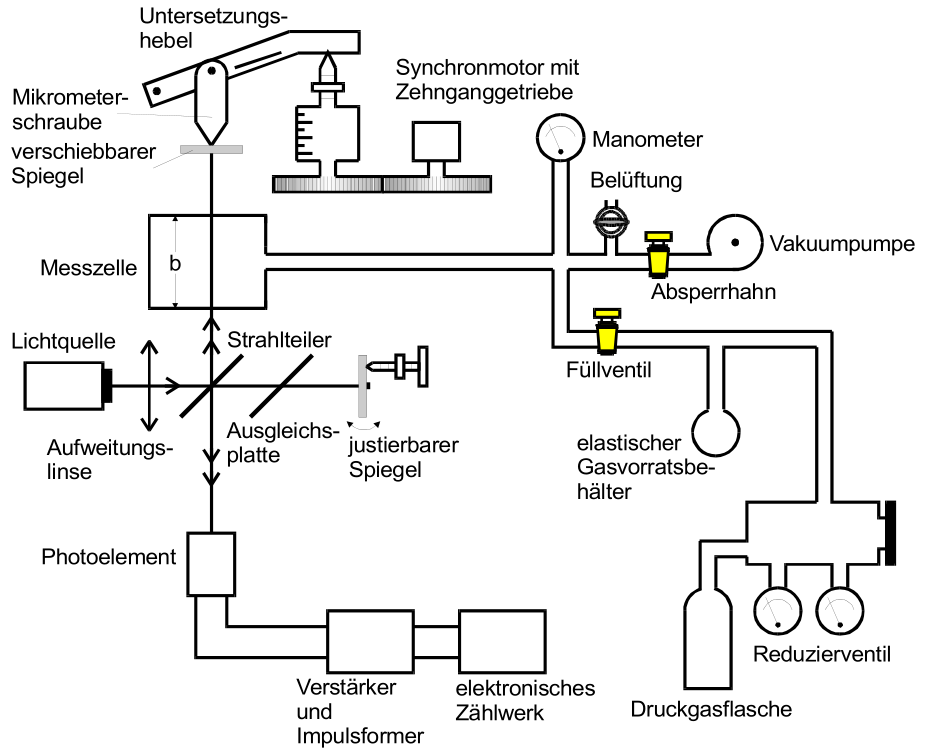
\includegraphics[width=0.5\textwidth]{build/Abb7.PNG}
    \caption {Aufbau des Experiments des Michelson-Interferometer \cite[3]{V401}.}
    \label{fig:Abb7}
\end{figure}
Damit Interferenzen beobachtet werden können, muss der Laserstrahl in zwei Teile aufgeteilt werden.
Dies geschieht indem das Licht auf eine semipermeable Platte fällt, welche als Strahlteiler fungiert.
Einer der Strahlwege kann durch einen beweglichen Spiegel, der durch einen Motor verschoben wird, verlängert werden.
Außerdem ist bei dem verstellbaren Weg eine Messzelle angebracht, welche eine Breite von $b=\qty{50}{\milli\meter}$ hat.
Diese lässt sich sowohl evakuieren, als auch mit verschiedenen Gasen befüllen, sodass durch
den geänderten Brechungsindex in der Messzelle ebenso ein optischer Wegunterschied
zwischen beiden Strahlwegen entsteht.
Im unbewegten Strahlweg ist zudem eine Ausgleichsplatte angebracht, da dieser Strahlweg im
Gegensatz zum anderen Strahlweg nicht dreimal, sondern nur einmal durch den in der
Mitte angebrachten Strahlteiler führt.
Die beiden Strahlwege enden beide auf dem Detektor, wo die Interferenzmaxima durch eine Schaltung mit einem elektronischem Zählwerk erfasst werden.

\section{Durchführung}
\label{sec:Durchführung}
Zu Beginn des Versuchs muss das Michelson-Interferometer für die Messung justiert werden. 
Dazu wird der Laser eingeschaltet und an die Position des Detektors ein weißes Blatt Papier, zur besseren Sichtbarkeit des Lasers, eingebracht.
Der justierbare Spiegel wird so ausgerichtet, dass die beiden hellsten Intensitätsmaxima
der beiden ankommenden Strahlen möglichst genau übereinander treffen. 
Der Detektor wird entsprechend so ausgerichtet, dass die Intensitätsmaxima beider
Strahlen genau auf dem Eintrittsspalt des Detektors liegen.\\
\\
Um die Wellenlänge des Lasers zu bestimmen, wird der verschiebare Spiegel benutzt. Dazu wird der Motor eingeschaltet und eine Verschieberichtung
ausgewählt.
In $10$ Messungen wird der Abstand $d$ des Spiegels mithilfe des Motors solange vergrößert bis ungefähr $2000$ Intensitätsmaxima durch das automatische
Zählwerk erfasst werden.
Wichtig ist, dass der Spiegel nicht zu schnell bewegt wird, sodass alle Intensitätsmaxima vom Detektor erfasst werden.
Nachdem etwa 2000 Intensitätsmaxima am Zähler abzulesen sind, wird die Messung gestoppt, die Anzahl der Intensitätsmaxima und die Verschiebestrecke 
des Motors abgelesen und in eine Tabelle notiert.
Mittels der Hebelübersetzung wird die Verschiebestrecke $\Delta d$ des Spiegels berechnet.
Die Messung wird zehnmal durchgeführt.\\
\\

Zur Bestimmung des Brechungsindex von Luft wird die Position des verschiebbaren Spiegels nicht
mehr verändert.
Die Messzelle wird mittels der Vakuumpumpe auf den Druck $p$ evakuiert, welcher notiert
wird. Beim langsamen Wiedereinlassen der Luft wird erneut die Anzahl der Intensitätsmaxima gezählt
und sobald wieder der Normaldruck $p0$ in der Messzelle herrscht, wird deren Anzahl z notiert.
Die Messung wird sechs Mal wiederholt.
